\paragraph{}
        Le projet PFA effectué est un projet d'imagerie numérique. Son but est de travailler à l'aide d'un logiciel dans une scène virtuelle en trois dimensions, et d'obtenir grâce à cette dernière des images en deux dimensions permettant de recréer une illusion de trois dimensions. Les algorithmes qui auront notamment été étudiés au cours de ce projet permettent l'obtention d'anaglyphes, d'autostéréogrammes, ou encore de folioscopes.
        L'imagerie numérique n'est pas étudiée au cours des deux premières années d'Informatique à l'Enseirb-Matmeca. Ainsi, ce projet constituait une réelle ouverture d'esprit sur un nouveau domaine de l'informatique.
        

//présentation anaglyphe
//présentation autostéréogramme
//présentation folioscope




\ref{fig:sphère}.

\begin{figure}[h]
	\centering
	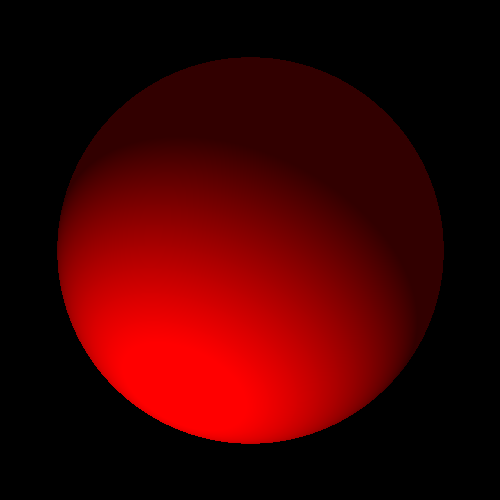
\includegraphics[scale=0.3]{boule.png}
	\caption{\label{fig:sphère} Application d’une lumière diffuse à une sphère rouge \protect \footnotemark }
\end{figure}
\footnotetext{http://linut.free.fr/omgspl0kuberwebloglolz0r/?2010/02/01/93-raytracer-que-la-lumiere-soit}

